\appendix

% \setcounter{page}{1}


% \setcounter{figure}{7}
% \setcounter{table}{3}
\newcommand{\refcolor}[1]{\textcolor{nvidiagreen}{#1}}



\section{Additional Experimental Setup}

\subsection{Algorithm}

\begin{algorithm}[H]
    \SetAlgoLined
    \caption{Training \ours{} (Sec.~\refcolor{3.2})}\label{algo:train}
    \KwIn{CoT-SFT checkpoint $\mathcal{F}_{\theta_0}$, training data $\mathcal{D}$, rollout size $N$, latent reasoning steps $M$, number of waypoints $K$, total iterations $T_{\text{total}}$}
    \KwOut{Trained student model $\mathcal{F}_\theta$}
    
    \tcp{Initialize models}
    $\mathcal{F}_\theta^T \leftarrow \mathcal{F}_{\theta_0}$, $\mathcal{F}_\theta \leftarrow \mathcal{F}_{\theta_0}$\;
    Initialize verbalizer $\mathcal{V}_\psi$ from pre-trained LLM\;
    $t \leftarrow 0$\;
    
    \While{$t < T_{\text{total}}$}{
        Sample batch $(o, l, \hat{p})$ from $\mathcal{D}$\;\tcp{Suppose bs=1 for simplicity}
        \vspace{0.5em}
        
        \tcp{Teacher GRPO training}
        Generate $N$ rollouts $\{\tau_i\}_{i=1}^N$ from $\mathcal{F}_\theta^T(o, l)$\;
        Compute trajectory rewards $\{r_i\}_{i=1}^N$\;
        Compute group-wise advantages $\{A_i\}_{i=1}^N$\;
        Update $\mathcal{F}_\theta^T$ with $\mathcal{J}_{\text{GRPO}}$ (Eq.~\refcolor{1})\;
        $\tau^+ \leftarrow \arg\max_i A_i$, $\tau^- \leftarrow \arg\min_i A_i$ (Eq.~\refcolor{3}) \tcp*{For student distillation}
        $h_t^T \leftarrow$ hidden state of $\tau^+$ at \texttt{<answer>} token from $\mathcal{F}_\theta^T$ \tcp*{For distillation loss}

        \vspace{0.5em}
        \tcp{Student latent distillation}
        $\mathbf{z} = \{z_m\}_{m=1}^M \leftarrow \mathcal{F}_\theta(o, l)$ \tcp*{Perform auto-regressive latent reasoning}
        Compute $\mathcal{L}_{\text{verb}}$ with $\mathbf{z}$, $\mathcal{V}_\psi$, $\tau^+$, $\tau^-$ (Eq.~\refcolor{4})\;
        
        Forward $K$ spatial tokens from $\mathcal{F}_\theta(o, l, \mathbf{z})$ to obtain $h_t$ and $\{h^\prime(\mathbf{s}_i)\}_{i=1}^K$\;
        Compute $\mathcal{L}_{\text{distill}}$ with $h_t^T$, $h_t$ (Eq.~\refcolor{5})\;
        Compute $\mathcal{L}_{\text{ans}}$ with $\{h^\prime(\mathbf{s}_i)\}_{i=1}^K$, $\hat{p}$ (Eq.~\refcolor{6})\;
        
        Update $\mathcal{F}_\theta$ with $\mathcal{L}_{\text{student}} = \mathcal{L}_{\text{verb}} + \mathcal{L}_{\text{distill}} + \mathcal{L}_{\text{ans}}$\;
        
        $t \leftarrow t + 1$\;
    }
    
    \Return{$\mathcal{F}_\theta$}\;
\end{algorithm}


Algorithm~\ref{algo:train} presents the complete training procedure corresponding to Sec.~\refcolor{3.2}. It shows how we jointly optimize the teacher model with GRPO and distill its reasoning into the student's compact latent representations.

\subsection{Implementation Details}

Our implementation follows the setup described in Sec.~\refcolor{4.1} of the main paper. Here we provide additional details. The verbalizer $\mathcal{V}_\psi$ is initialized from a small LLM, Qwen3-0.6B, with cross-attention layers inserted at each layer to condition on latent CoTs $\mathbf{z}$. For the student model training, in the first 3,000 iterations, we replace verbalization loss $\mathcal{L}_{\text{verb}}$ with language modeling loss using $\tau^+$ as ground truth to warm up $\mathcal{V}_\psi$'s alignment with the latent representations $\mathbf{z}$. We then freeze $\mathcal{V}_\psi$ and use the $\mathcal{L}_{\text{verb}}$ for the remaining 1,500 iterations. The student $\mathcal{F}_\theta$ is optimized throughout both phases. For waypoint prediction in Eq.~\refcolor{6}, each $p_i \in \mathbb{R}^6$ encodes coordinates in the format $[x_{\text{single}}, y_{\text{single}}, x_{\text{left}}, y_{\text{left}}, x_{\text{right}}, y_{\text{right}}]$, where the first two dimensions are for single-arm and the last four are for bimanual robot. For ground-truth $\hat{p}i$, we fill the corresponding dimensions based on robot type and mask out the unused dimensions when computing $\mathcal{L}_{\text{ans}}$. For GRPO training, we follow the configuration of ThinkAct~\cite{huang2025thinkact}, using rollout size $N=5$. Following~\cite{lee2025molmoact}, we set the number of waypoints in trajectory to $K=5$. We use $M=6$ latent reasoning tokens, with ablation study provided in Fig.~\ref{fig:supp:ablate_steps}.

During reasoning-enhanced policy learning, for SimplerEnv~\cite{li24simpler} evaluation, to ensure fair comparison with previous works~\cite{kim24openvla, lee2025molmoact}, we initialize $\pi_\phi$ from DiT-Policy~\cite{chi2023diffusion} pre-trained on the same OXE dataset~\cite{o2024open, kim24openvla} and conduct reasoning-enhanced policy learning (Sec.~\refcolor{3.3}) using the same OXE data. For LIBERO~\cite{liu2023libero} and RoboTwin2.0~\cite{chen2025robotwin2} evaluations, we initialize $\pi_\phi$ from RDT~\cite{liu2024rdt}, which has demonstrated strong performance on RoboTwin2.0, and conduct policy learning using OXE~\cite{o2024open} and static ALOHA datasets~\cite{shi2023waypoint, zhao2023learning}. Our method further enhances RDT's manipulation capabilities on both benchmarks. The use of different action models also demonstrates that our approach is agnostic to the underlying action model choice.


\subsection{Training Data Details}

\subsubsection{Dataset Sources}


\paragraph{2D Visual Trace of Manipulation Tasks.} For single-arm manipulation, we utilize 2D visual trajectories labeled by MolmoAct~\cite{lee2025molmoact} from the Open X-Embodiment (OXE) dataset~\cite{o2024open}, comprising approximately 1.3M trajectories. For bimanual manipulation, we extract dual-arm visual trajectories from the AIST dataset~\cite{aist2025aist}, resulting in approximately 92K trajectory samples. Specifically, we first use Molmo-72B~\cite{deitke2024molmo} to detect left and right gripper positions (following~\cite{lee2025molmoact}) in the first frame, then apply CoTracker3~\cite{karaev2025cotracker3} to track and parse the manipulation trajectories throughout the video sequences.

\paragraph{RoboFAC~\cite{lu2025robofac}.} RoboFAC is a robotic failure analysis dataset containing 9,440 erroneous manipulation trajectories across 16 tasks in both simulated and real-world environments. We utilize the training set with 64K QA pairs covering various failure types for developing failure identification and correction planning capabilities.

\paragraph{RoboVQA~\cite{sermanet2024robovqa}.} RoboVQA contains robot manipulation videos with QA tasks covering task understanding. The dataset includes approximately 5K long-horizon and 92K medium-horizon video sequences from diverse robotic platforms, resulting in total 798K QA pairs. Videos are annotated with multiple questions probing spatial reasoning, action prediction, and task comprehension.

\paragraph{ShareRobot~\cite{ji2025robobrain}.} ShareRobot is a large-scale dataset collected by RoboBrain~\cite{ji2025robobrain}, containing over 1M QA pairs covering task planning, object affordances, and manipulation strategies across diverse robot embodiments and scenes. The dataset features fine-grained annotations linking task descriptions to frame-level execution details, facilitating learning of transferable manipulation knowledge.

\paragraph{EgoPlan-Bench~\cite{chen2023egoplan}.} EgoPlan-Bench features egocentric videos of daily activities annotated with task planning information including goals, execution history, and current states. The dataset contains approximately 53K video-text pairs for training long-horizon planning and progress tracking capabilities from egocentric view.

\paragraph{Video-R1-CoT~\cite{feng2025video}.} Video-R1 comprises 165K video question-answer pairs with chain-of-thought reasoning annotations generated by large-scale vision-language models. The dataset covers diverse reasoning domains including mathematical logic, spatial understanding, OCR, and visual analytics. All samples are quality-filtered to ensure annotation consistency and correctness.

\paragraph{PixMo~\cite{deitke2024molmo}.} PixMo is a general-purpose vision-language dataset with diverse image captions and question-answer pairs. Following MolmoAct~\cite{lee2025molmoact}, we incorporate PixMo dataset to preserve general visual understanding and prevent catastrophic forgetting when training on embodied dataset. Specifically, we use approximately 726K samples from the \texttt{ask\_model\_anything}, \texttt{cap}, and \texttt{cap-qa} splits.

\subsubsection{Data Processing and Formatting}


\paragraph{Supervised Fine-Tuning (SFT).} To enhance foundational embodied knowledge, we perform supervised fine-tuning on approximately 4M samples combining 2D visual trajectories from MolmoAct~\cite{lee2025molmoact} and AIST~\cite{aist2025aist}, along with QA data from PixMo~\cite{deitke2024molmo}, RoboFAC~\cite{lu2025robofac}, RoboVQA~\cite{sermanet2024robovqa}, ShareRobot~\cite{ji2025robobrain}, and EgoPlan~\cite{chen2023egoplan}. This stage enables the model to acquire basic visual understanding, task comprehension, and manipulation knowledge across diverse embodiments and scenarios.

\paragraph{Chain-of-Thought SFT (CoT-SFT).} To develop reasoning capabilities while preserving embodied understanding, we sample 5\% from the SFT data (approximately 200K samples) and augment with 165K samples from Video-R1-CoT~\cite{feng2025video}. For data with CoT annotations, we format prompts to elicit structured reasoning enclosed in \texttt{<think>} tags followed by answers in \texttt{<answer>} tags; for data without CoT annotations, we prompt for direct answers only. This enables the model to learn reasoning capabilities from CoT-annotated data and generalize them to embodied tasks.

\paragraph{Teacher-Student Training.} Building upon the CoT-SFT checkpoint, we curate a balanced training set by sampling approximately 5,000 instances from each dataset and data type, totaling nearly 50K samples. We adopt the prompt formatting strategy from CoT-SFT for both teacher GRPO training and student latent distillation. We train both the teacher with GRPO and the student with latent distillation (as detailed in Sec.~\refcolor{3.2}) on this data, efficiently transferring high-quality reasoning patterns into compact latent representations.

\begin{table*}[t]
\centering
\caption{\textbf{Quantitative results with larger model size (7B or 8B) on embodied reasoning benchmarks.}}
\resizebox{1.0\textwidth}{!}{
\small
\begin{tabular}{lccccccccccccc}
\toprule
\textbf{Method} & \multicolumn{5}{c}{\textbf{EgoPlan-Bench2}} & \multicolumn{5}{c}{\textbf{RoboVQA}} & \textbf{OpenEQA} & \cellcolor{gray!15}\textbf{Overall} \\
\cmidrule(lr){2-6} \cmidrule(lr){7-11}
 & Daily. & Work. & Rec. & Hobbies & Avg. & B-1 & B-2 & B-3 & B-4 & B-Avg. & Score & \cellcolor{gray!15}Avg. \\
\midrule
InternVL2.5-8B~\cite{chen2024expanding} & 36.2 & 28.7 & 34.4 & 35.4 & 33.5 & 40.5 & 33.3 & 29.6 & 27.5 & 32.7 & 54.4 & \cellcolor{gray!15}40.2 \\
InternVL3-8B~\cite{zhu2025internvl3} & 38.5 & 32.9 & 36.1 & 37.2 & 36.2 & 44.3 & 36.5 & 31.6 & 28.9 & 35.3 & 55.5 & \cellcolor{gray!15}42.3 \\
NVILA-8B~\cite{liu2024nvila} & 35.8 & 28.7 & 37.2 & 35.4 & 33.7 & 42.7 & 39.7 & 37.6 & 36.1 & 39.0 & 54.0 & \cellcolor{gray!15}42.2 \\
Qwen2.5-VL-7B~\cite{bai2025qwen2} & 31.4 & 26.7 & 29.5 & 28.6 & 29.1 & 47.8 & 41.2 & 36.2 & 33.7 & 39.7 & 50.8 & \cellcolor{gray!15}39.9 \\
Magma-8B~\cite{yang2025magma} & 32.1 & 25.7 & 34.4 & 29.3 & 29.8 & 38.6 & 31.5 & 28.1 & 26.7 & 31.2 & 49.1 & \cellcolor{gray!15}36.7 \\
RoboBrain2.0-7B~\cite{team2025robobrain2} & 39.4 & 27.0 & 33.9 & 32.2 & 33.2 & 44.9 & 38.2 & 34.7 & 33.5 & 37.8 & 51.1 & \cellcolor{gray!15}40.7 \\
ThinkAct-7B~\cite{huang2025thinkact} & 50.1 & 49.8 & 44.8 & 45.2 & 48.2 & 69.1 & 61.8 & 56.0 & 52.4 & 59.8 & 56.2 & \cellcolor{gray!15}54.7 \\
\midrule
\ours{}-7B & 51.3 & 47.3 & 41.5 & 45.9 & 47.5 & 70.4 & 63.3 & 57.3 & 53.2 & 61.1 & 59.0 & \cellcolor{gray!15}\textbf{55.9} \\
\bottomrule
\end{tabular}
}
\label{tab:supp_er_7b}
\vspace{-2mm}
\end{table*}

\begin{table}[t!]
    \centering
    \caption{\textbf{Results on LIBERO and SimplerEnv benchmarks with additional ThinkAct-3B comparison.}}
    \resizebox{0.65\columnwidth}{!}{
        \small
        \begin{tabular}{lccc}
            \toprule
            \textbf{Method} & \textbf{LIBERO} & \textbf{SimplerEnv-Google} & \textbf{Latency ($\downarrow$)} \\
            \midrule
            OpenVLA-7B~\cite{kim24openvla} & 76.5 & 40.2 & N/A \\
            CoT-VLA-7B~\cite{zhao2025cot} & 83.9 & N/A & N/A \\
            ThinkAct-7B~\cite{huang2025thinkact} & 84.4 & 68.3 & 7513 \\
            MolmoAct-7B~\cite{lee2025molmoact} & 86.8 & 64.9 & 6723 \\
            \midrule
            ThinkAct-3B~\cite{huang2025thinkact} & 83.1 & 64.7 & 5674 \\
            \textbf{Fast-ThinkAct-3B} & \textbf{89.7} & \textbf{68.7} & \textbf{805 (\textcolor{YellowGreen}{$\downarrow$7.0$\times$})} \\
            \bottomrule
        \end{tabular}
    }
    \label{tab:supp_libero_simpler}
\end{table}
\begin{table}[t!]
    \centering
    \caption{\textbf{Comparison with efficient textual reasoning methods.}}
    \resizebox{0.75\linewidth}{!}{
        \begin{tabular}{lcccc}
            \toprule
            \makecell{\textbf{Method}} &
            \makecell{\textbf{EgoPlan-}\\\textbf{Bench2}} &
            \makecell{\textbf{RoboVQA}} &
            \makecell{\textbf{OpenEQA}} &
            \makecell{\textbf{Average}} \\
            \midrule
            Textual Teacher $\mathcal{F}_\theta^T$ & 41.7 & 58.2 & 49.4 & 49.8 \\
            $\mathcal{F}_\theta^T$ Inference w/o thinking & 42.7 & 55.0 & 41.7 & 46.5 \\
            $\mathcal{F}_\theta^T$ Inference w/ 6 textual tokens & 39.3 & 53.0 & 46.5 & 46.3 \\
            $\mathcal{F}_\theta^T$ w/ RL Length-Penalty~\cite{arora2025training} & 41.2 & 57.5 & 44.7 & 47.8 \\
            \midrule
            Fast-ThinkAct-3B & \textbf{46.4} & \textbf{60.8} & \textbf{52.8} & \textbf{53.3} \\
            \bottomrule
        \end{tabular}
    }
    \label{tab:supp:compare_efficient}
\end{table}



\subsection{Evaluation Setup}

\subsubsection{Embodied Reasoning Benchmarks}

We evaluate on three benchmarks assessing different aspects of embodied reasoning. EgoPlan-Bench2~\cite{chen2023egoplan} tests egocentric task planning across 24 daily-life scenarios with 1,321 multiple-choice questions, measuring accuracy in predicting next steps given task goals and progress history. RoboVQA~\cite{sermanet2024robovqa} evaluates visual reasoning in manipulation contexts through 1,893 free-form QA pairs from robot and human demonstrations, assessed via BLEU score. OpenEQA~\cite{majumdar2024openeqa} assesses spatial and functional understanding through 1,600+ questions spanning 180+ real-world environments, evaluated using LLM-based scoring aligned with human preferences. These benchmarks comprehensively evaluate embodied reasoning capability across planning, manipulation, and spatial understanding.

\subsubsection{Robotic Manipulation Benchmarks}

\begin{figure*}[t!]
    \centering
    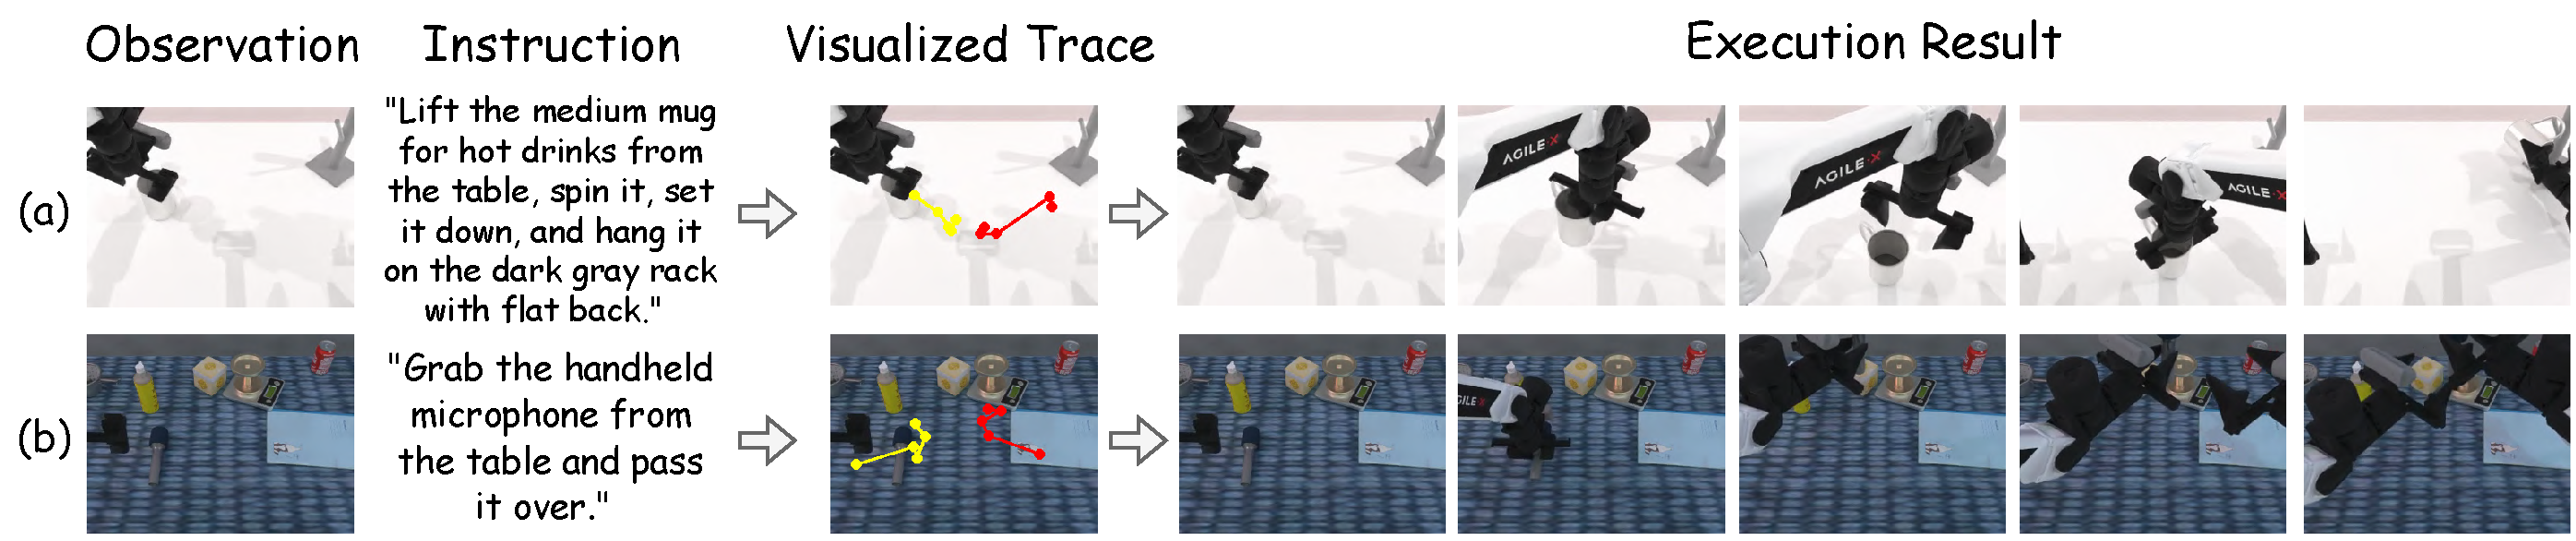
\includegraphics[width=0.96\linewidth]{figures/images/supp_visualize_manipulation.pdf}
    \caption{\textbf{Visualization of predicted visual trajectories and action execution results on RoboTwin2.0.} Yellow traces indicate left gripper trajectories; red traces indicate right gripper trajectories for bimanual tasks.}
    \vspace{-2mm}
    \label{fig:supp:visualize_manipulation}
\end{figure*}

\begin{figure*}[t!]
    \centering
    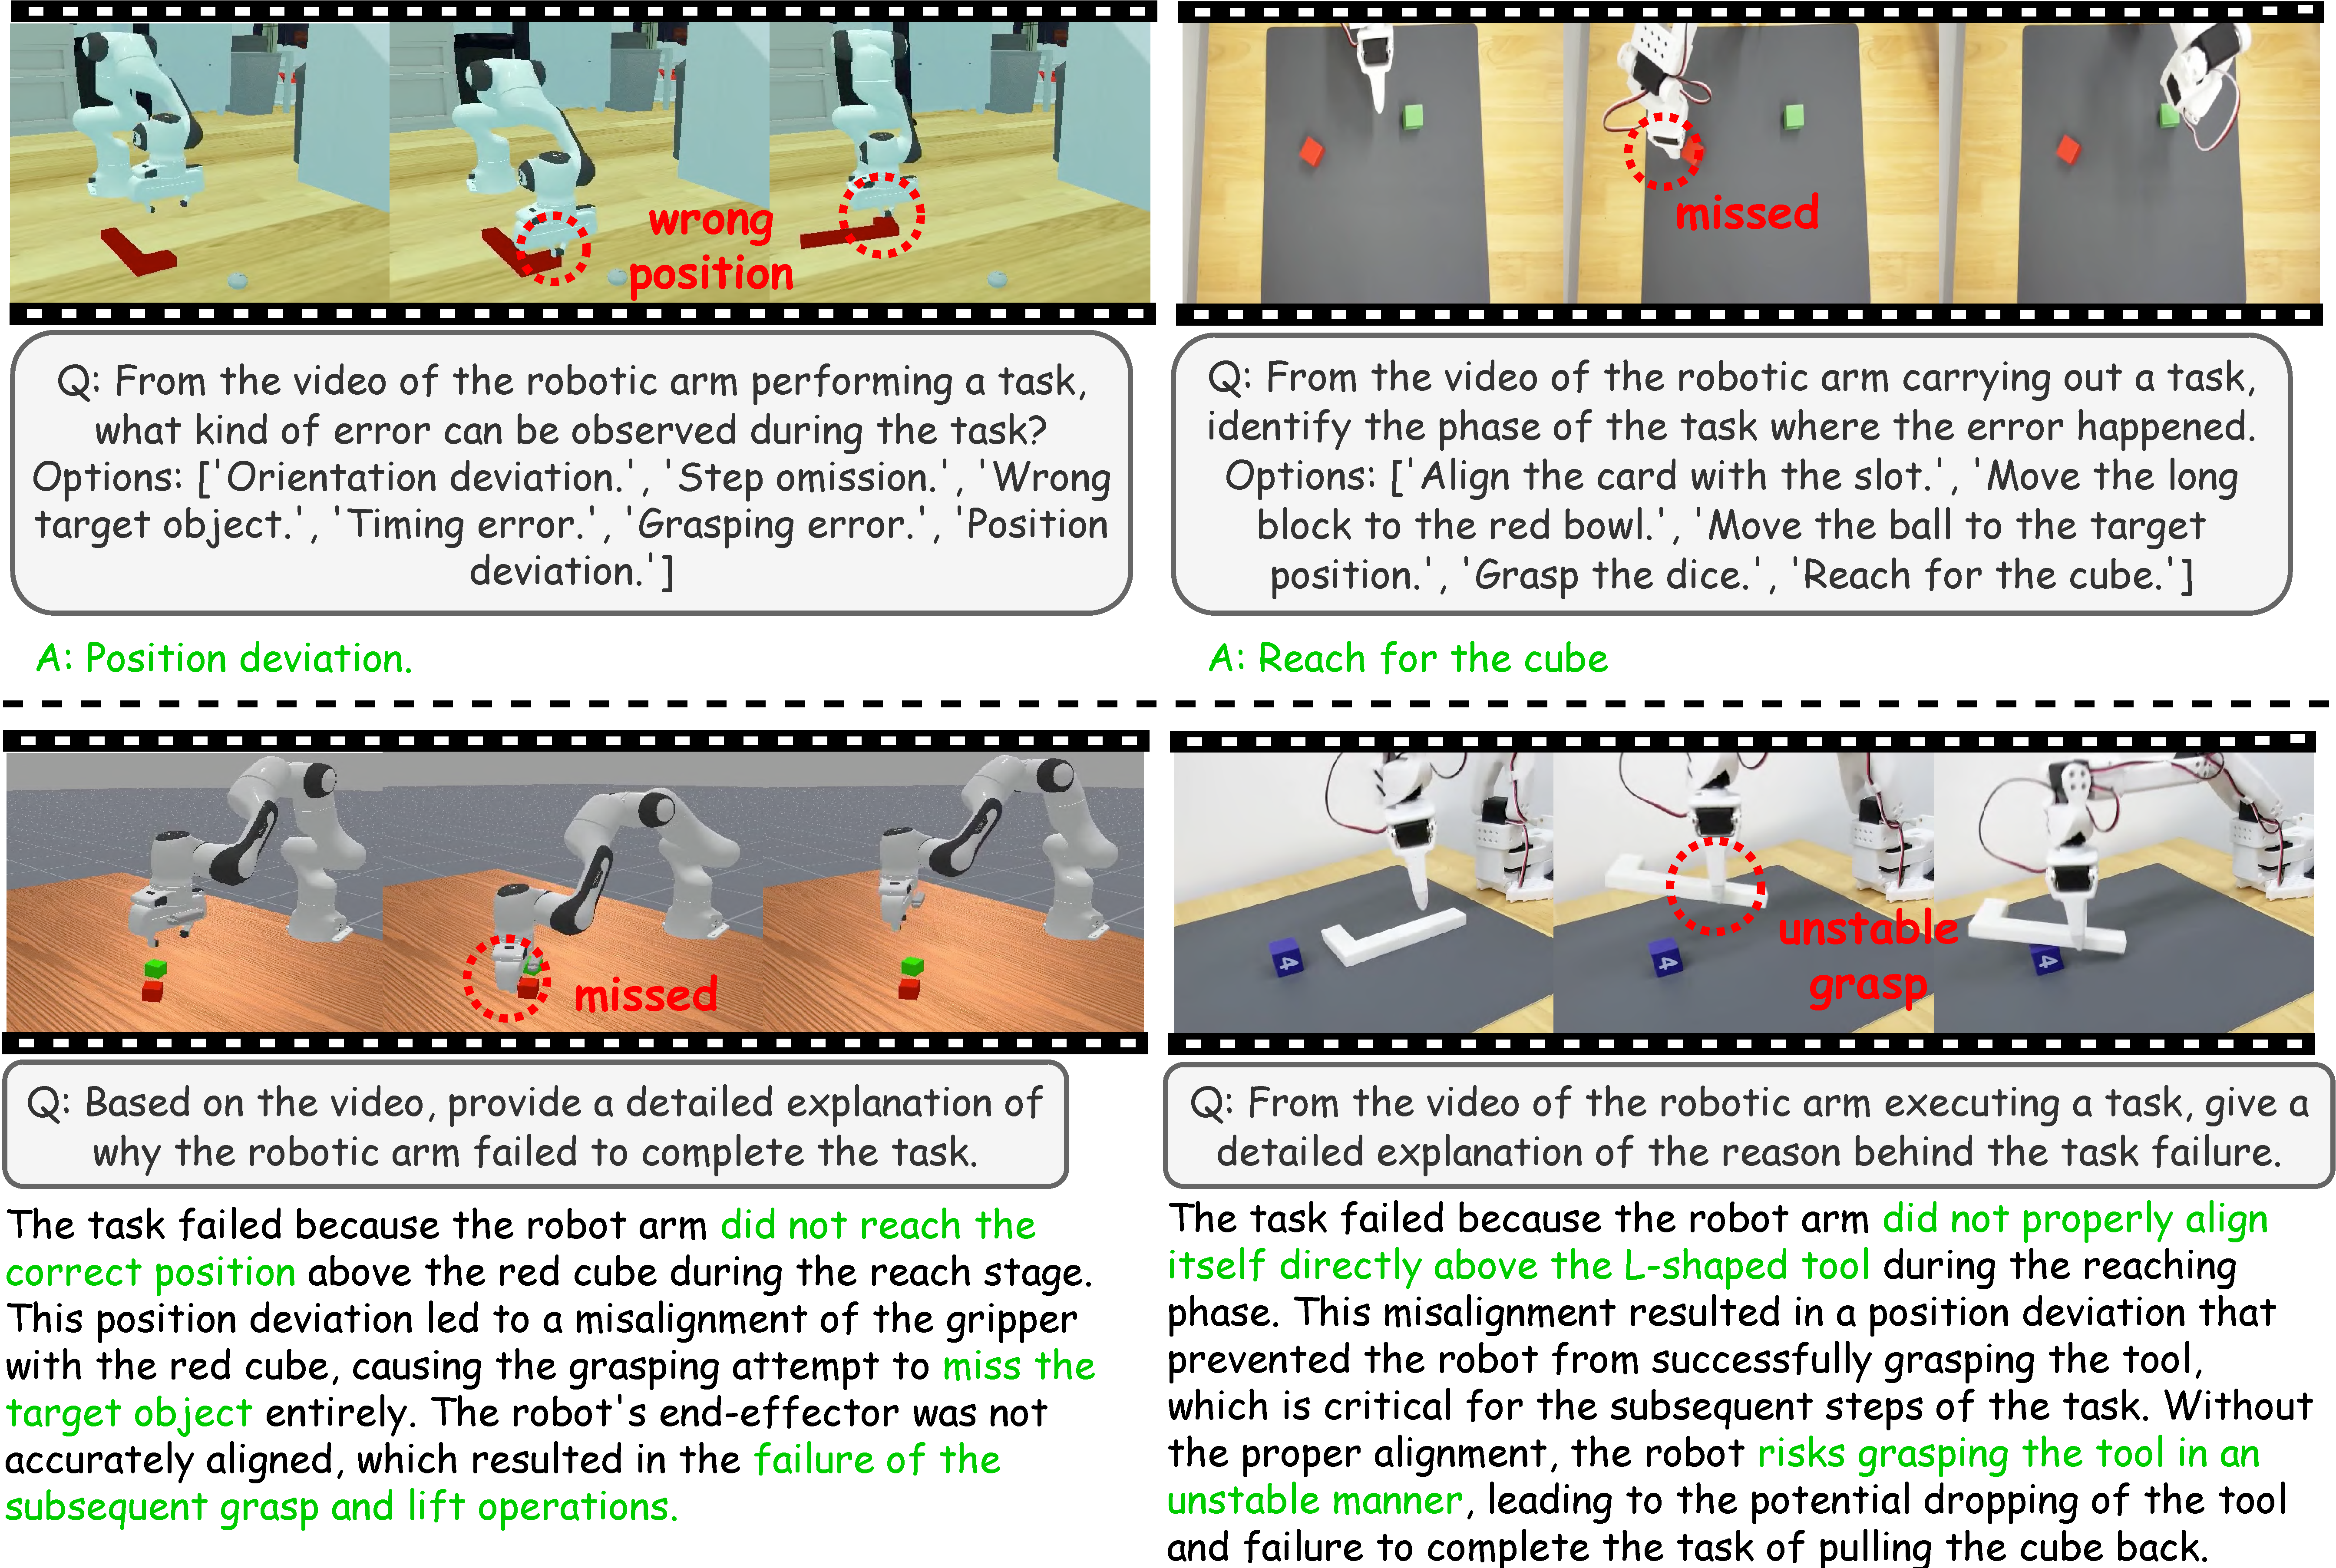
\includegraphics[width=0.9\linewidth]{figures/images/supp_visualize_robofac.pdf}
    \caption{\textbf{Failure identification and analysis capabilities on RoboFAC~\cite{lu2025robofac}.} Top row shows identification of failure types and execution stages. Bottom row demonstrates failure root cause analysis.}
    \label{fig:supp:visualize_robofac}
    % \vspace{-1mm}
\end{figure*}


\begin{figure}[t!]
    \centering
    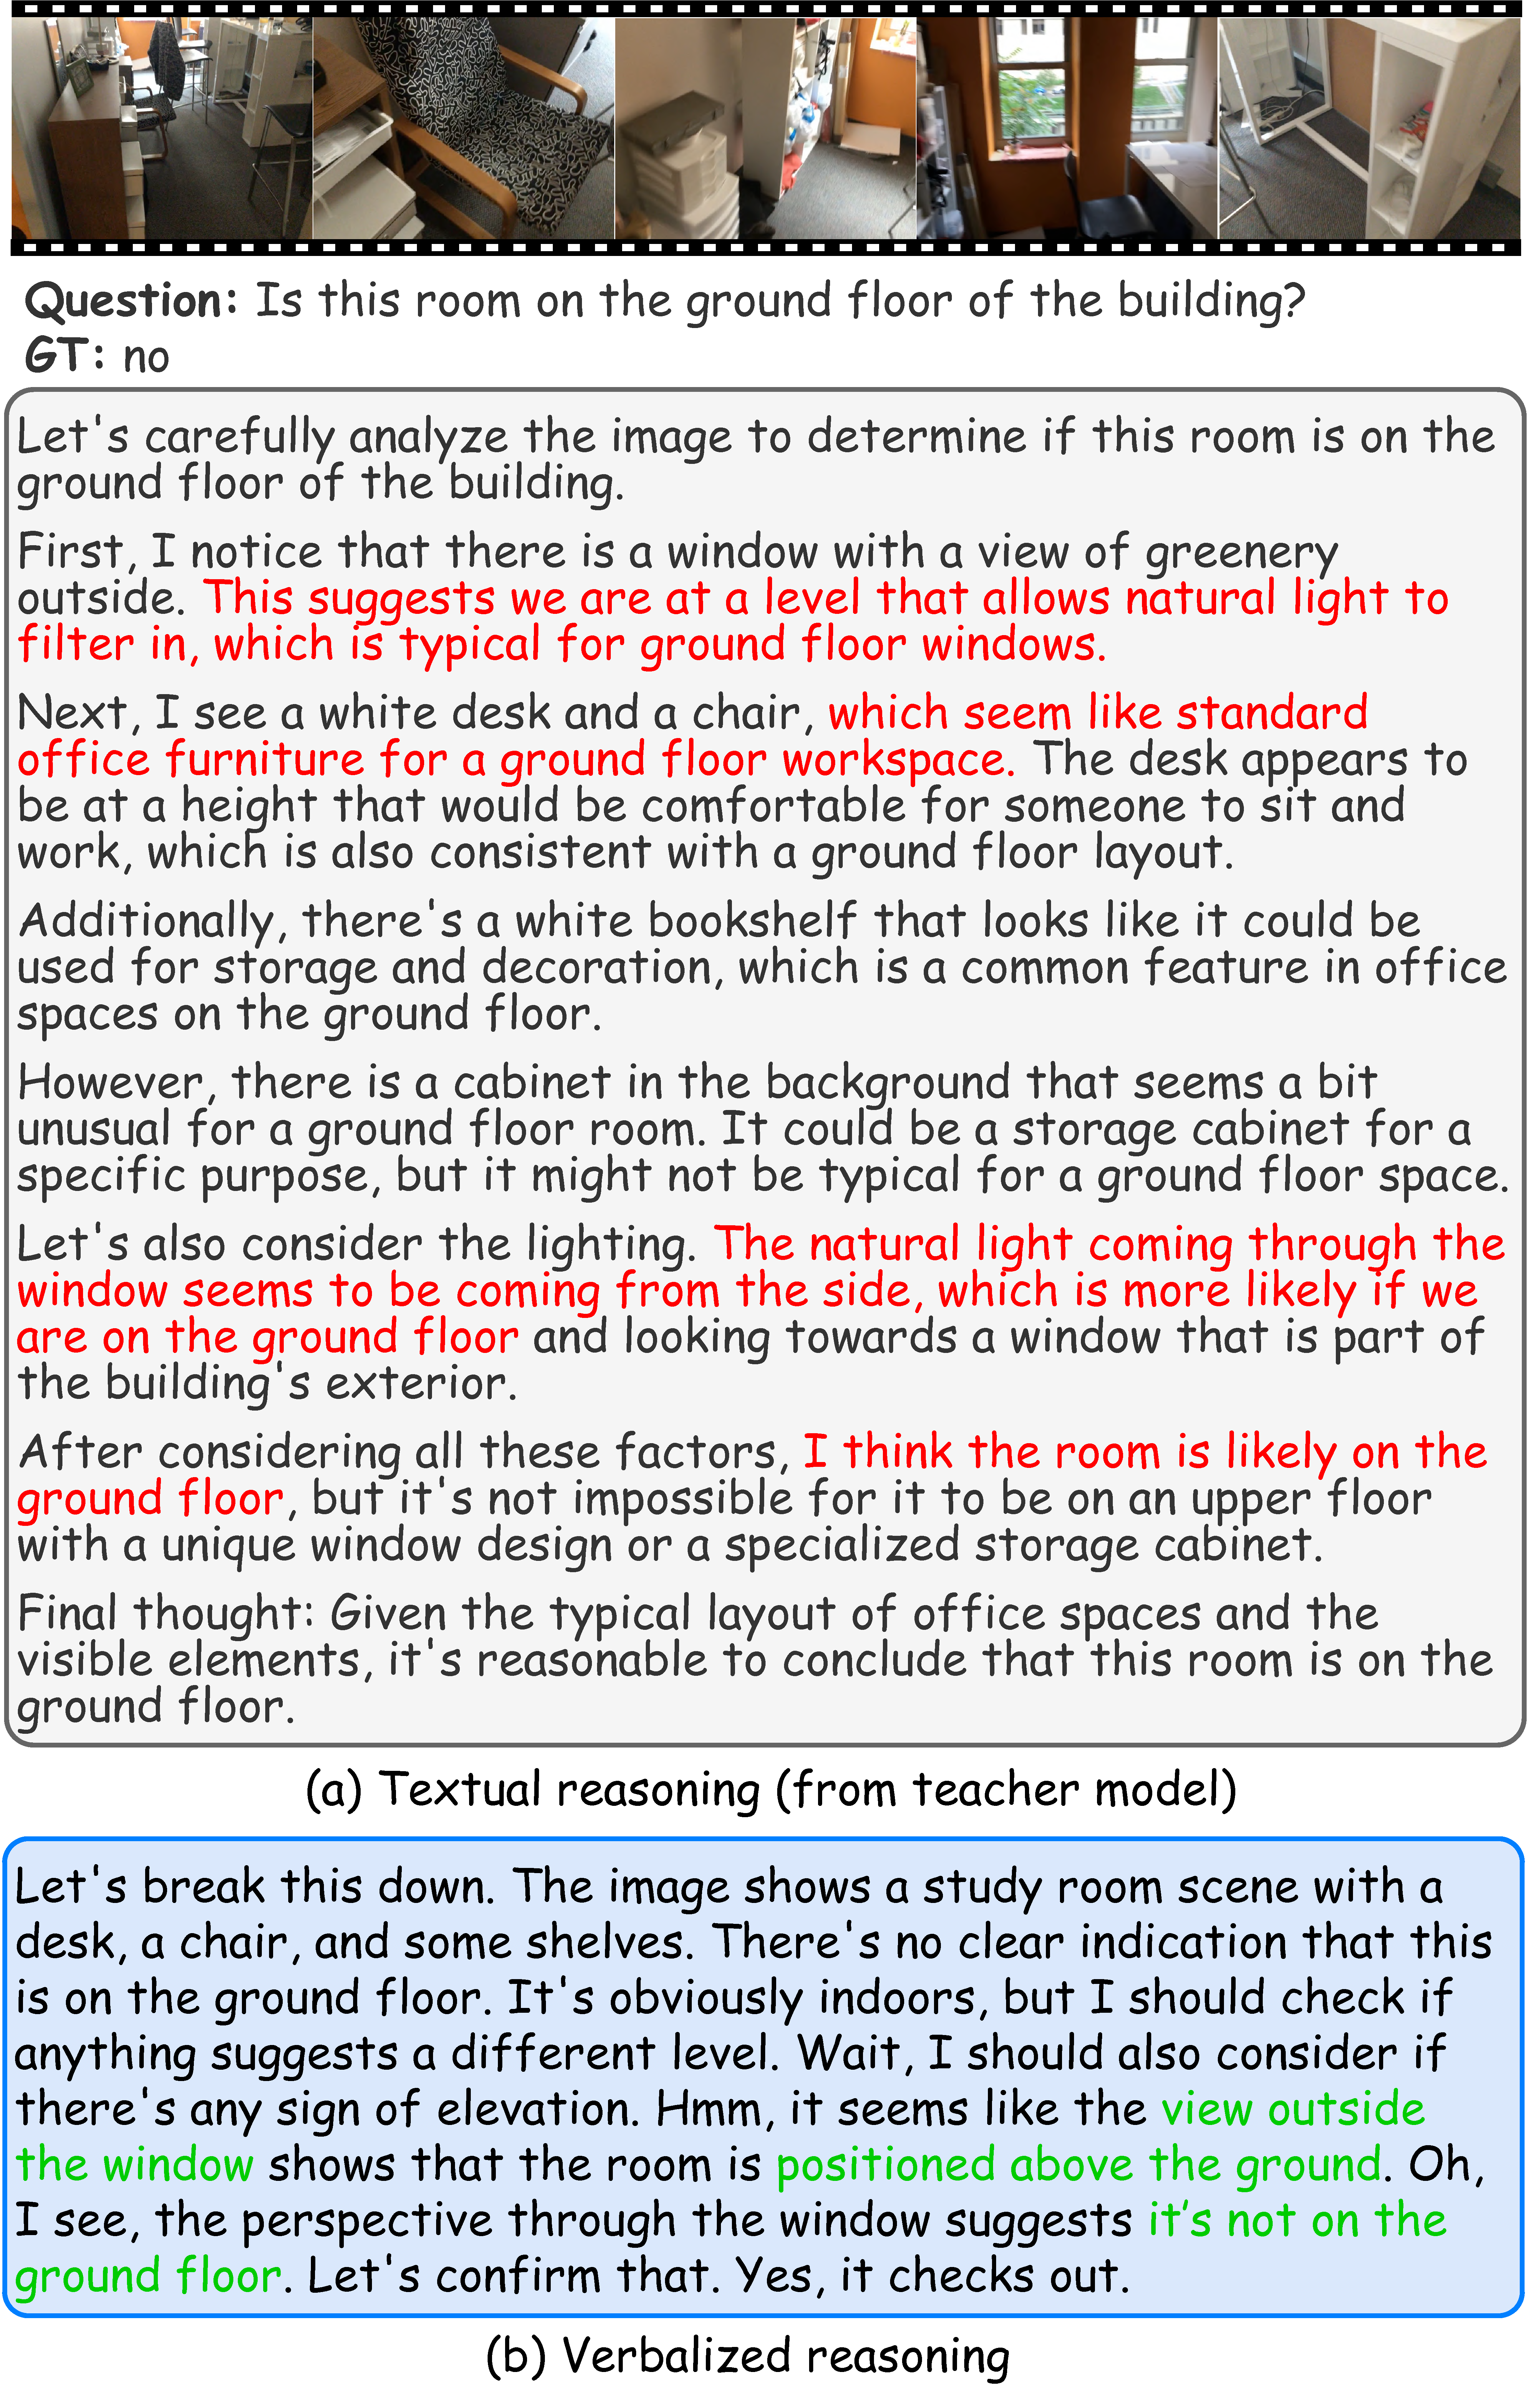
\includegraphics[width=0.60\linewidth]{figures/images/supp_visualize_reasoning.pdf}
    \caption{\textbf{Reasoning trace comparison on OpenEQA.} (a) Teacher's textual reasoning. (b) Student's verbalized latent reasoning. \textcolor{YellowGreen}{Green}: reasonable reasoning trace; \textcolor{red}{red}: incorrect trace.}
    \label{fig:supp:visualize_reasoning}
    % \vspace{-0.5mm}
\end{figure}


We evaluate on three simulation benchmarks covering diverse manipulation scenarios. SimplerEnv~\cite{li24simpler} provides manipulation tasks with strong sim-to-real correlation, featuring diverse visual variations in lighting, textures, backgrounds, and camera poses. Following MolmoAct~\cite{lee2025molmoact}, we evaluate on the Google Robot tasks using the standard protocol~\cite{kim24openvla, lee2025molmoact} of directly evaluating on SimplerEnv after training on OXE. LIBERO~\cite{liu2023libero} targets different generalization challenges through four task suites: spatial layout variation (LIBERO-Spatial), object diversity (LIBERO-Object), goal variation (LIBERO-Goal), and long-horizon planning with mixed variations (LIBERO-Long). We evaluate each suite over 500 trials using 3 random seeds following prior works~\cite{kim24openvla, lee2025molmoact}. RoboTwin2.0~\cite{chen2025robotwin2} features challenging bimanual manipulation with easy and hard difficulty settings, where the hard setting introduces domain randomization including clutter, lighting variations, diverse textures, and height changes. Following the original protocol, we train on 50 clean expert demonstrations per task and evaluate with 100 rollouts under both settings. We assess 10 tasks categorized into short, medium, and long horizons based on demonstration lengths.


\section{Additional Experiment Results}

\subsection{Additional Quantitative Results}


% \paragraph{}

\paragraph{Results of Larger Model Size.} To demonstrate the scalability of our approach, we apply Fast-ThinkAct to a larger backbone, Qwen2.5-VL-7B, and evaluate its performance on embodied reasoning benchmarks. As shown in Tab.~\ref{tab:supp_er_7b}, Fast-ThinkAct consistently achieves strong performance across EgoPlan-Bench2~\cite{qiu2024egoplan2}, RoboVQA~\cite{sermanet2024robovqa}, and OpenEQA~\cite{majumdar2024openeqa}, validating that our latent reasoning distillation method effectively scales to larger model backbones.

\paragraph{Performance Comparison with ThinkAct-3B.} Tab.~\ref{tab:supp_libero_simpler} presents detailed numerical results corresponding to Fig.~\refcolor{3} with additional ThinkAct-3B results. At the same 3B model size, Fast-ThinkAct achieves notable performance gains (89.7 vs. 83.1 on LIBERO, 68.7 vs. 64.7 on SimplerEnv-Google) while dramatically improving efficiency with \textbf{\textcolor{YellowGreen}{7$\times$}} faster inference (805ms vs. 5674ms).

\paragraph{Comparison with Efficient Reasoning Baselines.} Table~\ref{tab:supp:compare_efficient} compares our method with efficient textual reasoning alternatives applied to the textual teacher $\mathcal{F}_\theta^T$. We evaluate three baselines: removing reasoning during inference entirely (0 tokens), constraining the teacher to generate only 6 textual tokens during inference, and applying RL training with a length penalty~\cite{arora2025training} to encourage concise reasoning ($\sim$50 tokens). These achieve 46.5, 46.3, and 47.8 respectively, all degrading from the teacher's 49.8. In contrast, \ours{} uses only 6 latent tokens and achieves \textbf{53.3}, demonstrating superior efficiency and performance.


\subsection{Additional Qualitative Results}

\paragraph{Qualitative Robot Execution.} We provide qualitative robot execution comparisons between the base action model RDT~\cite{liu2024rdt} and \ours{} in the supplementary video \texttt{Fast-ThinkAct.mp4}. Our method shows substantial improvements on challenging robotic execution tasks, where reasoning capabilities provide better spatial understanding and coordination for successful manipulation.


\paragraph{Bimanual Manipulation Results.} In Fig.~\ref{fig:supp:visualize_manipulation}, we present visualized trajectories and execution results for \texttt{hanging mug} and \texttt{handover mic} tasks under easy and hard settings in RoboTwin2.0~\cite{chen2025robotwin2}. The hard setting includes different backgrounds and distractor objects. These examples show successful bimanual coordination where predicted waypoints accurately guide both grippers through the manipulation sequence, demonstrating Fast-ThinkAct's spatial reasoning ability across varied visual conditions.

\paragraph{Failure Identification and Recovery.} In Fig.~\ref{fig:supp:visualize_robofac}, we demonstrate Fast-ThinkAct's failure identification and analysis capabilities, complementing the recovery planning shown in the main paper. The top row shows that Fast-ThinkAct identifies failure types (e.g., position deviation) and execution stages (e.g., reaching for the cube). The bottom row illustrates root cause analysis, for instance, in the bottom-right example, the model correctly infers that the failure to push the cube with an L-shaped tool stems from an improper initial grasp. These results demonstrate Fast-ThinkAct's comprehensive understanding of manipulation failures beyond recovery planning.


\paragraph{Verbalized Latent Reasoning.} Fig.~\ref{fig:supp:visualize_reasoning} visualizes teacher textual reasoning and student verbalized reasoning. While the student generates compact and correct (\textcolor{YellowGreen}{green}) reasoning, the teacher's lengthy output sometimes contains erroneous steps (\textcolor{red}{red}) that might degrade the performance.


\subsection{Additional Ablation Study and Analysis}

\paragraph{Additional Ablation Results on Manipulation Benchmarks.} Table~\ref{tab:supp:ablation_stage_loss} shows ablation results on LIBERO~\cite{liu2023libero}, SimplerEnv-Google~\cite{li24simpler}, and RoboTwin2.0~\cite{chen2025robotwin2}. Removing $\mathcal{L}_{\text{verb}}$ or $\mathcal{L}_{\text{distill}}$ progressively degrades performance, confirming their contributions. Our full model consistently outperforms the textual teacher and models without teacher-student training (CoT-SFT, SFT only), demonstrating the benefits of compact latent reasoning distillation.

\begin{table}[t!]
    \begin{minipage}{0.5\columnwidth}
        
        \centering
        \caption{\textbf{Additional ablation study of training objectives and learning stages on robot manipulation benchmarks.}}
        \label{tab:supp:ablation_stage_loss}
    
        \centering
        \resizebox{\linewidth}{!}{
        \begin{tabular}{lcccc}
            \toprule
            \makecell{\textbf{Method}} &
            \makecell{\textbf{LIBERO}} &
            \makecell{\textbf{SimplerEnv}\\\textbf{Google}} &
            \makecell{\textbf{RoboTwin2.0}} &
            \makecell{\textbf{Average}} \\
            \midrule
            \textbf{Fast-ThinkAct} & \textbf{89.7} & \textbf{68.7} & \textbf{46.1} & \textbf{68.2} \\
            \midrule
            w/o $\mathcal{L}_\text{verb}$ & 88.6 & 67.3 & 44.9 & 66.9 \\
            w/o $\mathcal{L}_\text{verb},\mathcal{L}_\text{distill}$ & 86.3 & 65.7 & 42.6 & 64.9 \\
            \midrule
            Textual Teacher & 88.5 & 67.3 & 45.8 & 67.2 \\
            SFT + CoT-SFT & 87.2 & 65.8 & 43.3 & 65.4 \\
            SFT only & 86.9 & 64.5 & 42.8 & 64.7 \\
            \bottomrule
        \end{tabular}
    }

    \end{minipage}\hfill
    \begin{minipage}{0.46\columnwidth}

        \centering
        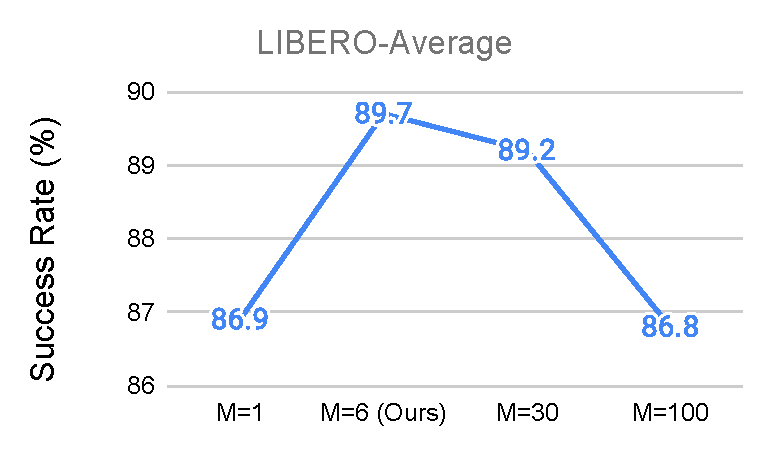
\includegraphics[width=\linewidth]{figures/images/supp_ablate_steps.pdf}

        \caption{\textbf{Ablation of Latent Reasoning Steps $M$.}}
    \label{fig:supp:ablate_steps}
    \end{minipage}

\end{table}



\paragraph{Ablation Study on Action Model Conditioning.} In Sec.~\refcolor{3.3}, we extract visual latent planning $c_t$ from early-layer KV cache of spatial tokens to condition the action model. We compare this against using late-layer KV cache (last $N$ layers, where $N$ is the action model depth) and directly using spatial tokens' output hidden states. Our approach achieves \textbf{89.7} on LIBERO, outperforming late-layer KV at 88.3 and output hidden states at 87.1, demonstrating that early-layer representations better capture visual planning information for action prediction. Therefore, we adopt early-layer KV conditioning as our default configuration.


\paragraph{Ablation Study on Latent Reasoning Steps.} In Fig.~\ref{fig:supp:ablate_steps}, we study the effect of latent reasoning steps $M$. We observe that too few steps ($M=1$) limit reasoning capacity, while excessive steps ($M=30, 100$) might introduce redundant or noisy information. Therefore, we adopt $M=6$, which achieves optimal performance, as our default.